\documentclass[
  lualatex, ja=standard, paper={182mm,257mm}, twocolumn, fontsize=8.5pt, baselineskip=13.5pt,
  line_length=24zw, column_gap=6.1mm, number_of_lines=45, head_space=24.5mm, gutter=16.25mm
]{jlreq}
\usepackage[haranoaji]{luatexja-preset}
\usepackage{luatexja-fontspec}
\setmainfont{TeX Gyre Termes}
\setsansfont{TeX Gyre Heros}
\usepackage{graphicx}
\usepackage{booktabs}
\usepackage{array}
\usepackage{xurl}
\urlstyle{same}
\usepackage[hidelinks]{hyperref}
\usepackage{fancyhdr}
\usepackage{microtype}
\usepackage{needspace}
\setlength{\parindent}{1\zw}
\setlength{\columnsep}{6.1mm}
\newcommand{\tablefont}{\fontsize{7.5pt}{10.5pt}\selectfont}
\renewcommand{\floatpagefraction}{0.7}
\renewcommand{\topfraction}{0.9}
\pagestyle{fancy}
\fancyhf{}
\renewcommand{\headrulewidth}{0pt}
\fancyfoot[L]{\fontsize{7.5pt}{9pt}\selectfont 教育情報分析研究会\hspace{1em}生成AI論文\hspace{1em}2026}
\fancyfoot[R]{\fontsize{9pt}{11pt}\selectfont\thepage}
\fancypagestyle{plain}{\fancyhf{}\renewcommand{\headrulewidth}{0pt}%
  \fancyfoot[L]{\fontsize{7.5pt}{9pt}\selectfont 教育情報分析研究会\hspace{1em}生成AI論文\hspace{1em}2026}\fancyfoot[R]{\fontsize{9pt}{11pt}\selectfont\thepage}}
\newcommand{\chap}[2]{\par\vspace{13.5pt}\needspace{4\baselineskip}{\centering\gtfamily\bfseries #1．#2\par}\nopagebreak}
\newcommand{\secn}[3]{\par\needspace{3\baselineskip}{\noindent\gtfamily\bfseries #1.#2.\hspace{1\zw}#3\par}\nopagebreak}
\newcommand{\chapspaced}[1]{\par\vspace{13.5pt}\needspace{4\baselineskip}{\centering\gtfamily\bfseries #1\par}\nopagebreak}

\begin{document}
\twocolumn[{%
\noindent\fbox{\parbox[c][16pt][c]{62mm}{\centering\gtfamily\fontsize{9pt}{16pt}\selectfont 生成AI論文}}\hfill{\fontsize{8pt}{12pt}\selectfont 教育情報分析研究会\hspace{1em}生成AI論文\hspace{1em}2026}\par
\vspace{14pt}{\centering\gtfamily\bfseries\fontsize{13pt}{20pt}\selectfont 具体物（操作教材）を使った算数・数学指導の効果：メタ分析\textsuperscript{†}\par}\vspace{10pt}
{\raggedleft\gtfamily\bfseries\fontsize{10pt}{15pt}\selectfont 教育情報分析研究会\hspace{4mm}\par}\vspace{10pt}
\begin{center}\parbox{\dimexpr\textwidth-12mm\relax}{\setlength{\parindent}{1\zw}操作教材とは，児童生徒が数学の考えを表すために手で扱う具体物やデジタル教具であり，その使用が学力の高さと関連するかを教師は知る必要がある．国内外のオープンアクセス論文から条件に合う８本 (参加者499人) を自動で選別・抽出し，数値を本文と照合したうえでランダム効果モデルにより統合した．統合値は \textit{g} = 1.49，95\%信頼区間 [0.97, 2.02]，\textit{I}² = 81.1\% であった．小規模な８件の研究では，操作教材を使った指導は事後テストの得点の高さと関連したが，効果のばらつきは大きく，証拠は予備的である．\par
{\gtfamily キーワード}：メタ分析，操作教材，算数・数学の学力，仮想操作教材，初等教育，前期中等教育\par}\end{center}\vspace{4pt}
}]
{\makeatletter\renewcommand{\thefootnote}{}\let\@makefnmark\@empty\footnotetext{\fontsize{7.5pt}{11pt}\selectfont 2026年10月11日公開}\makeatother}
\renewcommand{\thefootnote}{†}\footnotetext{\fontsize{7.5pt}{11pt}\selectfont Society for Educational Data Analysis (SEDA)：Effects of Concrete and Virtual Manipulatives on Mathematics Learning in Primary and Lower Secondary Students: A Meta-Analysis}
\chap{1}{はじめに}
小学校・中学校の算数・数学は，具体的な量から記号による表記へと進むが，抽象的な考えをつかみにくい児童生徒は多い．そのため教師は，数学の考えを目に見えて扱いやすくする方法をしばしば探している．

操作教材 (manipulatives) とは，児童生徒が数学の考えを表すために手で扱い動かす具体物やデジタル教具である．具体的な操作教材にはプラスチックのキューブや分数のタイルがあり (LIGGETT 2017，MAGTO and SALAZAR 2025)，仮想操作教材 (virtual manipulatives) は，幾何や代数のアプレットなどの対話的なデジタル教具である (EJIOFOR-CHIMA 2025，MAHMUTI and ARIFI 2025，TEMÜR and SEVIMLI 2024)．採用した研究は，分数 (MAGTO and SALAZAR 2025，UKDEM and ÇETİN 2022)，幾何 (CARCUEVA \textit{et al.} 2025，EJIOFOR-CHIMA 2025，MAHMUTI and ARIFI 2025，SCIPPO \textit{et al.} 2025)，代数 (TEMÜR and SEVIMLI 2024) などの内容でこれらを調べていた．

各研究は少数の学級と特定の内容を対象としているため，１件の研究からは限られた姿しか分からない．量的な統合 (quantitative synthesis) では，結果を同じ尺度にそろえ，群間の差の典型的な大きさを推定し，研究間で結果がどれだけ異なるかを示し，その差が小学校と中学校で異なるかを調べることができる．

本メタ分析の目的は，１〜９年生において，具体的または仮想的な操作教材を使って学んだ児童生徒と，使わずに学んだ児童生徒との間の算数・数学の学力の差を，全体として推定することであった．研究上の問いは，操作教材を使った指導と使わない指導とで事後テストの学力の差はどの程度か，またその差は学校段階によって異なるか，である．

\chap{2}{方法}
\secn{2}{1}{文献の検索}
2026年10月11日に，公開されている２つの書誌データベースを検索した．OpenAlex では題名と要旨を対象に次の検索式を用いた：「(manipulatives OR “concrete materials” OR “virtual manipulatives” OR “hands-on”) AND (mathematics OR math OR arithmetic OR geometry) AND (elementary OR primary OR “middle school” OR “junior high” OR “lower secondary” OR grade OR children OR pupils)」．対象は2012年以降に刊行されたオープンアクセスの学術誌論文で，分野が教育学 (Education) または発達・教育心理学 (Developmental and Educational Psychology) に分類されたものに限った．国内の研究を含めるため，J-STAGE でも要旨を対象に「具体物 算数」，「操作活動 算数 効果」のキーワードで検索した (2012年以降)．

\secn{2}{2}{適格基準}
次の条件をすべて満たす研究を対象とした：(a) 対象者：１〜９年生 (小学校・中学校) の児童生徒 (年齢はおよそ６〜15歳)．幼児のみ，高校生のみ，大学生，成人，教員・教員養成課程の学生の標本は除く；(b) 扱う要因：具体的または仮想的な操作教材を使った指導；(c) 比較の対象：操作教材を使わない指導 (例：記号的な指導，教科書のみの指導) ；(d) 成果指標：算数・数学の学力テスト；(e) 標準化平均差を計算できる統計量を報告していること．レビュー，質的研究，一事例実験，比較群のない前後比較のみの研究は除外した．

\secn{2}{3}{選別とデータの抽出}
選別とデータの抽出は言語モデル (gemma4:12b (Ollama; drafts) and claude-sonnet-5-5 (Claude Code; review and revision)) で行った．最初のモデル (Ollama) が，各論文の題名と要旨を適格基準に照らして評価した (この選別は確認していない)．評価の高い論文から本文 (PDF) を取得してテキストに変換し，同じモデルが研究の特徴と要約統計量の下書きを作った．そのうえで，２つ目のモデル (Claude Code) が，下書きを全文と照らして確認・修正し，適格かどうかも判断した．抽出したすべての数値は，本文にその数字が実際に書かれているかをプログラムで照合し，１つでも見つからない研究は統合から除外した．比較群の条件が，受動的 (介入なし・待機・通常授業) か能動的 (同じ成果を目指す別の介入) かも同じモデルが分類し，その根拠となる本文の箇所を引用させた．引用が本文に見つからない分類は「不明」とした．選別と抽出を人が確認する工程はない．条件を満たす研究が10本を超えた場合は，評価の高い10本を用いた．

\secn{2}{4}{効果量}
標準化平均差として Hedges の g を求めた (HEDGES 1981)．事後テストの平均・標準偏差・人数から計算し，それらが報告されていない場合は独立な２群の t 値，分子の自由度が１の F 値，報告された d または g の順に用いた．正の値は介入群の得点が高いことを表す．１研究につき１つの効果量を用いた．

\secn{2}{5}{統計解析}
効果量はランダム効果モデルで統合し，研究間分散 (\textit{τ}²) は DerSimonian–Laird 法で推定した (DERSIMONIAN and LAIRD 1986)．統合値の信頼区間と検定には，研究数が少ない場合に推奨される Hartung–Knapp–Sidik–Jonkman 法 (HKSJ 法) を用いた (HARTUNG and KNAPP 2001，INTHOUT \textit{et al.} 2014)．異質性は Q，\textit{I}² (HIGGINS and THOMPSON 2002)，\textit{τ}²，95\% 予測区間で評価した．学校段階 (小学校：１〜６年，中学校：７〜９年) ごとに２研究以上ある場合は下位集団分析を行った．比較条件の種類 (受動的・能動的) による下位集団分析も，各種類に２研究以上ある場合に行った (比較の種類が不明な研究は，この分析からのみ除いた)．頑健性は１研究ずつ除いた分析で確かめ，Egger の回帰検定 (EGGER \textit{et al.} 1997) は研究数が10以上の場合にのみ行うこととした．効果の大きさは慣例的な目安で解釈した (COHEN 1988)．計算は標準的な式 (BORENSTEIN \textit{et al.} 2009) に従い，公開した JavaScript のプログラム (\url{https://github.com/k518-2026/MetaAnalysisToWP}) で行った．

\chap{3}{結果}
\secn{3}{1}{研究の選定}
検索の結果，OpenAlex から200件 (検索式に合う1009件のうち上位)，J-STAGE から11件を得た．重複を除くと206件であった．要旨のある200件を選別し，27件を適格の可能性ありと判定した．本文を調べた27件のうち，取得または読み取りができなかったものが12件，適格基準を満たさなかったものが６件，統計量が不足していたものが０件，抽出した数値を本文で確認できなかったものが０件，効果量が現実的でない値になったものが１件であった．最終的に８本の研究をメタ分析に含めた．

\secn{3}{2}{研究の特徴}
対象とした研究 (CARCUEVA \textit{et al.} 2025，EJIOFOR-CHIMA 2025，LIGGETT 2017，MAGTO and SALAZAR 2025，MAHMUTI and ARIFI 2025，SCIPPO \textit{et al.} 2025，TEMÜR and SEVIMLI 2024，UKDEM and ÇETİN 2022) の国，学年，研究デザイン，人数，効果量を表１に示す．参加者は合計499人で，実施国はトルコ，イタリア，コソボ，カナダ，フィリピン，ナイジェリアであった．学校段階別では，小学校 (１〜６年) が３本，中学校 (７〜９年) が５本であった．１研究あたりの人数は32〜120人，研究ごとの効果量は \textit{g} = 0.68 から \textit{g} = 2.33 まで分布していた．

\begin{table*}[tb]
\centering
{\tablefont \gtfamily 表１\hspace{1em}対象とした研究の概要\par}\vspace{2pt}
{\tablefont\renewcommand{\arraystretch}{1.12}
\begin{tabular}{>{\raggedright\arraybackslash}p{0.2600\dimexpr\textwidth-12\tabcolsep\relax}>{\raggedright\arraybackslash}p{0.1100\dimexpr\textwidth-12\tabcolsep\relax}>{\raggedright\arraybackslash}p{0.1200\dimexpr\textwidth-12\tabcolsep\relax}>{\raggedright\arraybackslash}p{0.2300\dimexpr\textwidth-12\tabcolsep\relax}>{\raggedright\arraybackslash}p{0.0700\dimexpr\textwidth-12\tabcolsep\relax}>{\raggedright\arraybackslash}p{0.2100\dimexpr\textwidth-12\tabcolsep\relax}}
\toprule
研究 & 国 & 学年 & デザイン & \textit{N} & \textit{g} [95\% CI] \\
\midrule
UKDEM and ÇETİN (2022) & トルコ & 小学3年 & 準実験（実験群2・統制群1） & 41 & 1.42 [0.74, 2.09] \\
SCIPPO \textit{et al.} (2025) & イタリア & 小学4年 & 準実験 & 35 & 0.68 [0.02, 1.35] \\
MAHMUTI and ARIFI (2025) & コソボ & 中学1年 & 準実験 & 32 & 1.05 [0.33, 1.77] \\
LIGGETT (2017) & カナダ & 小学2年 & ランダム化比較試験 & 43 & 1.59 [0.92, 2.27] \\
TEMÜR and SEVIMLI (2024) & トルコ & 中学1年 & 準実験 & 60 & 1.61 [1.04, 2.19] \\
MAGTO and SALAZAR (2025) & フィリピン & 中学1年 & 準実験 & 84 & 0.83 [0.38, 1.27] \\
EJIOFOR-CHIMA (2025) & ナイジェリア & 中学3年 & 準実験 & 120 & 2.33 [1.87, 2.80] \\
CARCUEVA \textit{et al.} (2025) & フィリピン & 中学1年 & 準実験 & 84 & 2.31 [1.76, 2.86] \\
\bottomrule
\end{tabular}\par}
\vspace{2pt}{\tablefont\noindent 注：CI＝信頼区間．g は Hedges の g（正の値は介入群が高い）．学年・デザインは論文の本文から自動で抽出した．\par}
\end{table*}
各研究の介入，比較の条件，成果指標を表２に示す．８本はいずれも，介入群と比較群を事後テストで比べた研究である．

\begin{table*}[tb]
\centering
{\tablefont \gtfamily 表２\hspace{1em}各研究の介入・比較の条件・成果指標\par}\vspace{2pt}
{\tablefont\renewcommand{\arraystretch}{1.12}
\begin{tabular}{>{\raggedright\arraybackslash}p{0.2000\dimexpr\textwidth-8\tabcolsep\relax}>{\raggedright\arraybackslash}p{0.3200\dimexpr\textwidth-8\tabcolsep\relax}>{\raggedright\arraybackslash}p{0.2400\dimexpr\textwidth-8\tabcolsep\relax}>{\raggedright\arraybackslash}p{0.2400\dimexpr\textwidth-8\tabcolsep\relax}}
\toprule
研究 & 介入 & 比較の条件 & 成果指標 \\
\midrule
UKDEM and ÇETİN (2022) & 具体物の操作教材を使った分数指導（実験1） & 算数の教育課程にそった従来の指導 [受動] & 分数理解テスト（事後） \\
SCIPPO \textit{et al.} (2025) & GeoGebraと3Dプリント教材によるテッセレーションの指導 & 通常の幾何の授業（平面図形と角） [受動] & 幾何の学習テスト（事後） \\
MAHMUTI and ARIFI (2025) & 仮想操作用具を用いた指導 & 伝統的な指導法 [受動] & 周りと面積に関する事後テストのスコア \\
LIGGETT (2017) & プラスチック製のユニフィックス・キューブを使用した指導 & マニピュラティブ（操作用具）を使用しない指導 [受動] & 算数の学力テストのスコア \\
TEMÜR and SEVIMLI (2024) & 仮想操作用具を用いた活動ベースの指導 & 教科書を用いた活動 [受動] & 代数誤概念特定テスト \\
MAGTO and SALAZAR (2025) & 物理的な操作教材（分数円、棒、タイル、および演算タイル）を用いた指導 & 対照群 & 数学の達成度テスト（有理数の演算） \\
EJIOFOR-CHIMA (2025) & バーチャル・マニピュラティブを用いた指導（Right Triangle SolverおよびPythagorean theoryアプリレット） & 講義形式の指導 [受動] & 幾何学達成度テスト（GAT） \\
CARCUEVA \textit{et al.} (2025) & 操作用具を用いた指導 & 伝統的な指導 [受動] & 40項目の達成度テスト \\
\bottomrule
\end{tabular}\par}
\vspace{2pt}{\tablefont\noindent 注：論文の本文から自動で抽出し，要約した． [受動]＝介入なし・通常授業など，[能動]＝同じ成果を目指す別の介入．分類が不明なものは印を付けていない．\par}
\end{table*}
\secn{3}{3}{全体の効果}
図１に各研究の効果量と統合値をフォレストプロットで示す．四角は各研究の効果量で，大きさは統合における重みを表す．横線は95\%信頼区間，最下段のひし形は統合値である．８本のうち８本で効果量が正の値であり，８本では95\%信頼区間が０を含まなかった．重みが最も大きかったのは MAGTO and SALAZAR (2025) (13.7\%) であった．

\begin{figure*}[tb]
\centering
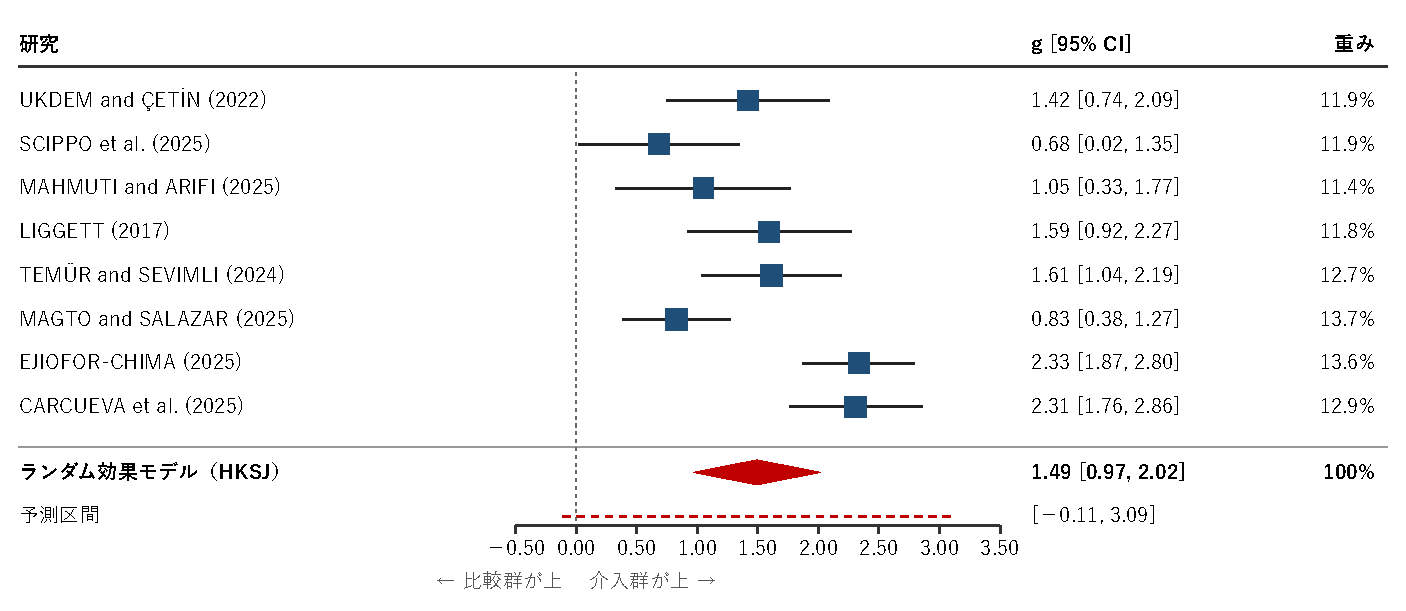
\includegraphics[width=\textwidth]{forest-ja.pdf}\par\vspace{2pt}
{\tablefont\gtfamily 図１\hspace{1em}フォレストプロット\par}{\tablefont 注：四角は各研究の効果量 (大きさは重み)，横線は95\%信頼区間，ひし形は統合値，点線は予測区間を表す．\par}
\end{figure*}
ランダム効果モデルによる統合値は \textit{g} = 1.49，95\% 信頼区間 [0.97, 2.02]，\textit{t}(7) = 6.70，p < .001 であった．慣例的な目安では大きい効果にあたる．固定効果モデルによる推定値は \textit{g} = 1.53 であった．これらの推定値を表３にまとめる．

\secn{3}{4}{異質性}
研究間の異質性は非常に大きかった (\textit{Q}(7) = 37.04，p < .001，\textit{I}² = 81.1\%，\textit{τ}² = 0.370)．95\% 予測区間は \ensuremath{-}0.11 から 3.09 であった．

\secn{3}{5}{下位集団分析と感度分析}
小学校 (１〜６年) では \textit{g} = 1.23，95\% 信頼区間 [0.03, 2.43] (\textit{k} = 3)，中学校 (７〜９年) では \textit{g} = 1.64，95\% 信頼区間 [0.77, 2.51] (\textit{k} = 5) であり，学校段階間の差は統計的に有意ではなかった (\textit{Q}(1) = 0.94，\textit{p} = .333)．比較条件の種類 (受動的・能動的) による下位集団分析は，少なくとも一方の種類で研究が２本未満だったため行わなかった．１研究ずつ除いた推定値は 1.36 から 1.60 の範囲であった．研究数が10未満のため，出版バイアスの検定は行わなかった．下位集団ごとの推定値も表３に示す．

\begin{table*}[tb]
\centering
{\tablefont \gtfamily 表３\hspace{1em}メタ分析の結果\par}\vspace{2pt}
{\tablefont\renewcommand{\arraystretch}{1.12}
\begin{tabular}{lrrrrrrr}
\toprule
モデル & \textit{k} & \textit{N} & \textit{g} & 95\% CI & \textit{p} & \textit{I}² (\%) & \textit{τ}² \\
\midrule
ランダム効果（HKSJ） & 8 & 499 & 1.49 & [0.97, 2.02] & < .001 & 81.1 & 0.370 \\
固定効果 & 8 & 499 & 1.53 & [1.33, 1.74] & < .001 & — & — \\
\hspace{1em}小学校（1〜6年） & 3 & 119 & 1.23 & [0.03, 2.43] & .048 & 49.9 & 0.118 \\
\hspace{1em}中学校（7〜9年） & 5 & 380 & 1.64 & [0.77, 2.51] & .006 & 86.5 & 0.478 \\
\bottomrule
\end{tabular}\par}
\vspace{2pt}{\tablefont\noindent 注：\textit{k}＝研究数．HKSJ＝Hartung–Knapp–Sidik–Jonkman 法による信頼区間．95\% 予測区間 [\ensuremath{-}0.11, 3.09]．\par}
\end{table*}
\chap{4}{考察}
ランダム効果モデルによる統合した差は，操作教材を使った指導に有利な大きなものであった (\textit{g} = 1.49，95\% 信頼区間 [0.97, 2.02]，p < .001)  (表３)．８件すべての研究で効果は正であり，その範囲は \textit{g} = 0.68 (SCIPPO \textit{et al.} 2025) から \textit{g} = 2.33 (EJIOFOR-CHIMA 2025) であった (図１)．この大きさの効果は慎重に読む必要がある．研究の規模は小さく (N は32から120)，無作為に割り付けた研究は１件だけであり (LIGGETT 2017)，ほかは既存の学級どうしを事後テストで比べていたため，授業の前からあった群間の差や学級間のその他の違いが結果に影響した可能性がある．

結果は研究間で大きくばらついた (図１)．異質性は大きく (\textit{I}² = 81.1\%，\textit{τ}² = 0.370)，95\% 予測区間 [\ensuremath{-}0.11, 3.09] には，０に近い値も非常に大きな値も含まれる．このため，統合値を特定の教室で期待できる利益とみなしてはならない．研究間では，操作教材の種類 (具体物，仮想，またはデジタルと３Dプリントを組み合わせたプログラム (SCIPPO \textit{et al.} 2025))，内容と学年，成果指標のテストが異なっており (表２)，今回のデータからは，これらのうちどれが違いを説明するのかは分からない．

学校段階別の分析では，小学校の標本 (\textit{k} = 3) で \textit{g} = 1.23，95\% 信頼区間 [0.03, 2.43]，中学校の標本 (\textit{k} = 5) で \textit{g} = 1.64，95\% 信頼区間 [0.77, 2.51] であった．学校段階間の差は統計的に有意ではなく (\textit{Q}(1) = 0.94，\textit{p} = .333)，これらの結果は探索的で，少数の研究に基づく．受動的な比較条件と能動的な比較条件の比較はできなかった．７件の研究は操作教材を通常の指導または従来の指導と比べており (CARCUEVA \textit{et al.} 2025，EJIOFOR-CHIMA 2025，LIGGETT 2017，MAHMUTI and ARIFI 2025，SCIPPO \textit{et al.} 2025，TEMÜR and SEVIMLI 2024，UKDEM and ÇETİN 2022)，１件は比較の内容を述べていなかったためである (MAGTO and SALAZAR 2025)．１件ずつ研究を除いて統合し直した推定値は1.36から1.60の間であり，１件の研究だけが全体の結果を決めたわけではなかった．出版バイアスは，研究が10件未満のため評価できなかった．

１〜９年生の教師にとって，これらの結果は，たとえば分数 (MAGTO and SALAZAR 2025，UKDEM and ÇETİN 2022)，幾何 (CARCUEVA \textit{et al.} 2025，EJIOFOR-CHIMA 2025，MAHMUTI and ARIFI 2025，SCIPPO \textit{et al.} 2025)，代数 (TEMÜR and SEVIMLI 2024) で，具体的な操作教材や仮想の操作教材を試す価値があることを示している．ただし，これらの研究は操作教材だけで学力が上がることを示してはおらず，ここで報告された差の大きさがどの学級でも再現されるとは考えにくい．分かりやすい説明とあわせて操作教材を使い，自分の学級で児童生徒の理解が深まるかを確かめるのが妥当である．

\chap{5}{まとめ}
２〜９年生を対象とした小規模な８件の研究では，具体的または仮想的な操作教材を使った指導は，使わない指導より事後テストの算数・数学の得点が高いことと関連していた (\textit{g} = 1.49)．ただし研究間の差は大きく，予測区間には０に近い値も含まれる．多くの研究が小規模な準実験であるため，この結果は予備的である．これは，教師が操作教材を試して自分の学級での効果を確かめる理由にはなるが，操作教材がこの大きさだけ学力を高めることを証明するものではない．

本統合にはいくつかの限界がある．採用した研究は８件のみで，標本の大きさは32から120であり，８件のうち７件は既存の学級を対象とした準実験研究で，無作為化した研究は１件だけであった (LIGGETT 2017)．事後テストの得点を用いたため，授業前の群間差は調整していない．介入，比較条件 (多くは「従来の指導」「通常の指導」としか書かれておらず，１件ではまったく書かれていなかった (MAGTO and SALAZAR 2025))，内容，成果指標のテストが異なるため，統合値はおおまかな要約にとどまる．小規模な研究は大きな効果を示しやすく，出版バイアスは評価できなかった．

データは全文から自動で抽出し，すべての抽出を人が確かめたわけではない．全文を入手できなかった，または統計量を確実に読み取れなかったために，採用できなかった候補の研究もいくつかあった．加えて，効果が不自然に大きかった１件の研究は，抽出の誤りの可能性が高いとしてソフトウェアが除外した．これらの理由から，本知見は暫定的なものとして扱うべきである．

加えて，本分析は選別とデータ抽出を言語モデルで行った．選別は確認しておらず，抽出した数値は，本文との文字列の照合と，２つ目のモデルによる全文との突き合わせで確かめたが，人による確認は経ていない．数値が本文に存在し，確認を通っても，別の群や別の測定の値を取り違えている可能性は残る．対象はオープンアクセスで本文を取得できた論文に限られ，有料の論文や未刊行の研究は含まれていない．

\chapspaced{付\hspace{1\zw}記}
本論文は，教育情報分析研究会が生成AIを用いて自動で作成した「生成AI論文」である．文献の選別，データの抽出，はじめに・考察・まとめの文章の作成には大規模言語モデル (gemma4:12b (Ollama; drafts) and claude-sonnet-5-5 (Claude Code; review and revision)) を用い，統計量はすべてプログラムで計算した．査読は受けていない．

同じ内容の英語版がある (\url{https://raw.githubusercontent.com/k518-2026/MetaAnalysisToWP/main/reports/2026-10-11-math-manipulatives/paper-en.pdf})．抽出したデータとプログラムは \url{https://github.com/k518-2026/MetaAnalysisToWP} で公開している．

\chapspaced{参考文献}
{\noindent * はメタ分析に含めた研究を示す．\par}
{\small
\par\noindent\hangindent=2\zw\hangafter=1 BORENSTEIN, M., HEDGES, L. V., HIGGINS, J. P. T. and ROTHSTEIN, H. R. (2009) \textit{Introduction to Meta-Analysis}. Wiley. \url{https://doi.org/10.1002/9780470743386}\par
\par\noindent\hangindent=2\zw\hangafter=1 *CARCUEVA, C. E., BASMAYOR, B. B., BOISER, R. D., RABADON, G. F. and SAAVEDRA, R. T. (2025) IMPACT OF MANIPULATIVE-BASED INSTRUCTION ON STUDENTS’ CONCEPTUAL UNDERSTANDING OF BASIC GEOMETRY IN A SECONDARY SCHOOL. \textit{European Journal of Education Studies}, \textbf{12} (11). \url{https://doi.org/10.46827/ejes.v12i11.6409}\par
\par\noindent\hangindent=2\zw\hangafter=1 COHEN, J. (1988) \textit{Statistical Power Analysis for the Behavioral Sciences} (2nd ed.). Lawrence Erlbaum Associates\par
\par\noindent\hangindent=2\zw\hangafter=1 DERSIMONIAN, R. and LAIRD, N. (1986) Meta-analysis in clinical trials. \textit{Controlled Clinical Trials}, \textbf{7} (3)：177-188. \url{https://doi.org/10.1016/0197-2456(86)90046-2}\par
\par\noindent\hangindent=2\zw\hangafter=1 EGGER, M., DAVEY SMITH, G., SCHNEIDER, M. and MINDER, C. (1997) Bias in meta-analysis detected by a simple, graphical test. \textit{BMJ}, \textbf{315} (7109)：629-634. \url{https://doi.org/10.1136/bmj.315.7109.629}\par
\par\noindent\hangindent=2\zw\hangafter=1 *EJIOFOR-CHIMA, N. A. (2025) Effect of Visual Manipulatives on Junior Secondary School Students’ Interest and Achievement in Geometry. \textit{Faculty of Natural and Applied Sciences Journal of Mathematics and Science Education}. \url{https://fnasjournals.com/index.php/FNAS-JMSE/article/view/701}\par
\par\noindent\hangindent=2\zw\hangafter=1 HARTUNG, J. and KNAPP, G. (2001) A refined method for the meta-analysis of controlled clinical trials with binary outcome. \textit{Statistics in Medicine}, \textbf{20} (24)：3875-3889. \url{https://doi.org/10.1002/sim.1009}\par
\par\noindent\hangindent=2\zw\hangafter=1 HEDGES, L. V. (1981) Distribution theory for Glass's estimator of effect size and related estimators. \textit{Journal of Educational Statistics}, \textbf{6} (2)：107-128. \url{https://doi.org/10.3102/10769986006002107}\par
\par\noindent\hangindent=2\zw\hangafter=1 HIGGINS, J. P. T. and THOMPSON, S. G. (2002) Quantifying heterogeneity in a meta-analysis. \textit{Statistics in Medicine}, \textbf{21} (11)：1539-1558. \url{https://doi.org/10.1002/sim.1186}\par
\par\noindent\hangindent=2\zw\hangafter=1 INTHOUT, J., IOANNIDIS, J. P. A. and BORM, G. F. (2014) The Hartung-Knapp-Sidik-Jonkman method for random effects meta-analysis is straightforward and considerably outperforms the standard DerSimonian-Laird method. \textit{BMC Medical Research Methodology}, \textbf{14}：25. \url{https://doi.org/10.1186/1471-2288-14-25}\par
\par\noindent\hangindent=2\zw\hangafter=1 *LIGGETT, R. (2017) The Impact of Use of Manipulatives on the Math Scores of Grade 2 Students. \textit{Brock Education Journal}, \textbf{26} (2). \url{https://doi.org/10.26522/brocked.v26i2.607}\par
\par\noindent\hangindent=2\zw\hangafter=1 *MAGTO, R. Y. and SALAZAR, P.  D. A. (2025) Tangible Mathematics for Grade 7 Learners: Design and Validation of Manipulatives for Rational Number Concepts. \textit{International Journal on Science and Technology}, \textbf{16} (2). \url{https://doi.org/10.71097/ijsat.v16.i2.3255}\par
\par\noindent\hangindent=2\zw\hangafter=1 *MAHMUTI, A. and ARIFI, A. (2025) Integration of Virtual Manipulatives for Teaching and Learning Perimeter and Area in Lower Secondary Education. \textit{Innovaciencia Facultad de Ciencias Exactas Físicas y Naturales}, \textbf{13} (1). \url{https://doi.org/10.15649/2346075x.5051}\par
\par\noindent\hangindent=2\zw\hangafter=1 *SCIPPO, S., MADIAI, S. and CUOMO, S. (2025) Digital Tessellation for Geometry Learning in Primary School: A Quasi-Experimental Study. \textit{Journal of Information Technology Education Research}, \textbf{24}：009. \url{https://doi.org/10.28945/5473}\par
\par\noindent\hangindent=2\zw\hangafter=1 *TEMÜR, T. and SEVIMLI, E. (2024) Investigation of the Effect of Virtual Manipulatives Usage on the Process of Eliminating Misconceptions about Algebraic Expressions and Equations. \textit{Uluslararası Türk Eğitim Bilimleri Dergisi}, \textbf{12} (2)：805-852. \url{https://doi.org/10.46778/goputeb.1434000}\par
\par\noindent\hangindent=2\zw\hangafter=1 *UKDEM, S. and ÇETİN, H. (2022) INVESTIGATING THE IMPACT OF INTERVENTIONS USING CONCRETE AND VIRTUAL MANIPULATIVES ON 3 TH GRADE STUDENTS' FRACTION CONCEPT AND MOTIVATION:. \textit{International online journal of education and teaching}. \url{https://iojet.org/index.php/IOJET/article/view/1674}\par
}
\chapspaced{Summary}
{\setlength{\parindent}{1\zw}\noindent Manipulatives are objects and digital tools that students handle to represent mathematical ideas, and teachers need to know whether using them is linked to higher achievement. Using an automated workflow in which every extracted number was verified against the full text, 8 open-access studies (\textit{N} = 499) were pooled with a random-effects model. The pooled effect was \textit{g} = 1.49, 95\% CI [0.97, 2.02], with \textit{I}² = 81.1\%. In these eight small studies, instruction with manipulatives was associated with higher post-test scores, but the effects varied widely, so the evidence is preliminary.\par
KEYWORDS: META-ANALYSIS, MANIPULATIVES, MATHEMATICS ACHIEVEMENT, VIRTUAL MANIPULATIVES, PRIMARY EDUCATION, LOWER SECONDARY EDUCATION\par}
\end{document}
